\section{最急降下法と共役勾配法}

\begin{frame}[t,fragile]{最急降下法(steepest-descent)}
  \begin{itemize}
    %\setlength{\itemsep}{1em}
  \item 関数の微分の情報を使う
  \item 現在の点$\bf x$における勾配を計算
    \[
    -\nabla f|_i = -\frac{\partial f}{\partial x_i}
    \]
  \item 坂を下る方向にそって、一次元最適化
  \item 動いた先の勾配の方向でさらに最適化を繰り返す
  \item 関数値は単調減少 $\Rightarrow$ 極小値に収束
  \end{itemize}
\end{frame}

\begin{frame}[t,fragile]{細長い谷の場合}
  \vspace*{1em}
  \hspace*{1em}\resizebox{1\textwidth}{!}{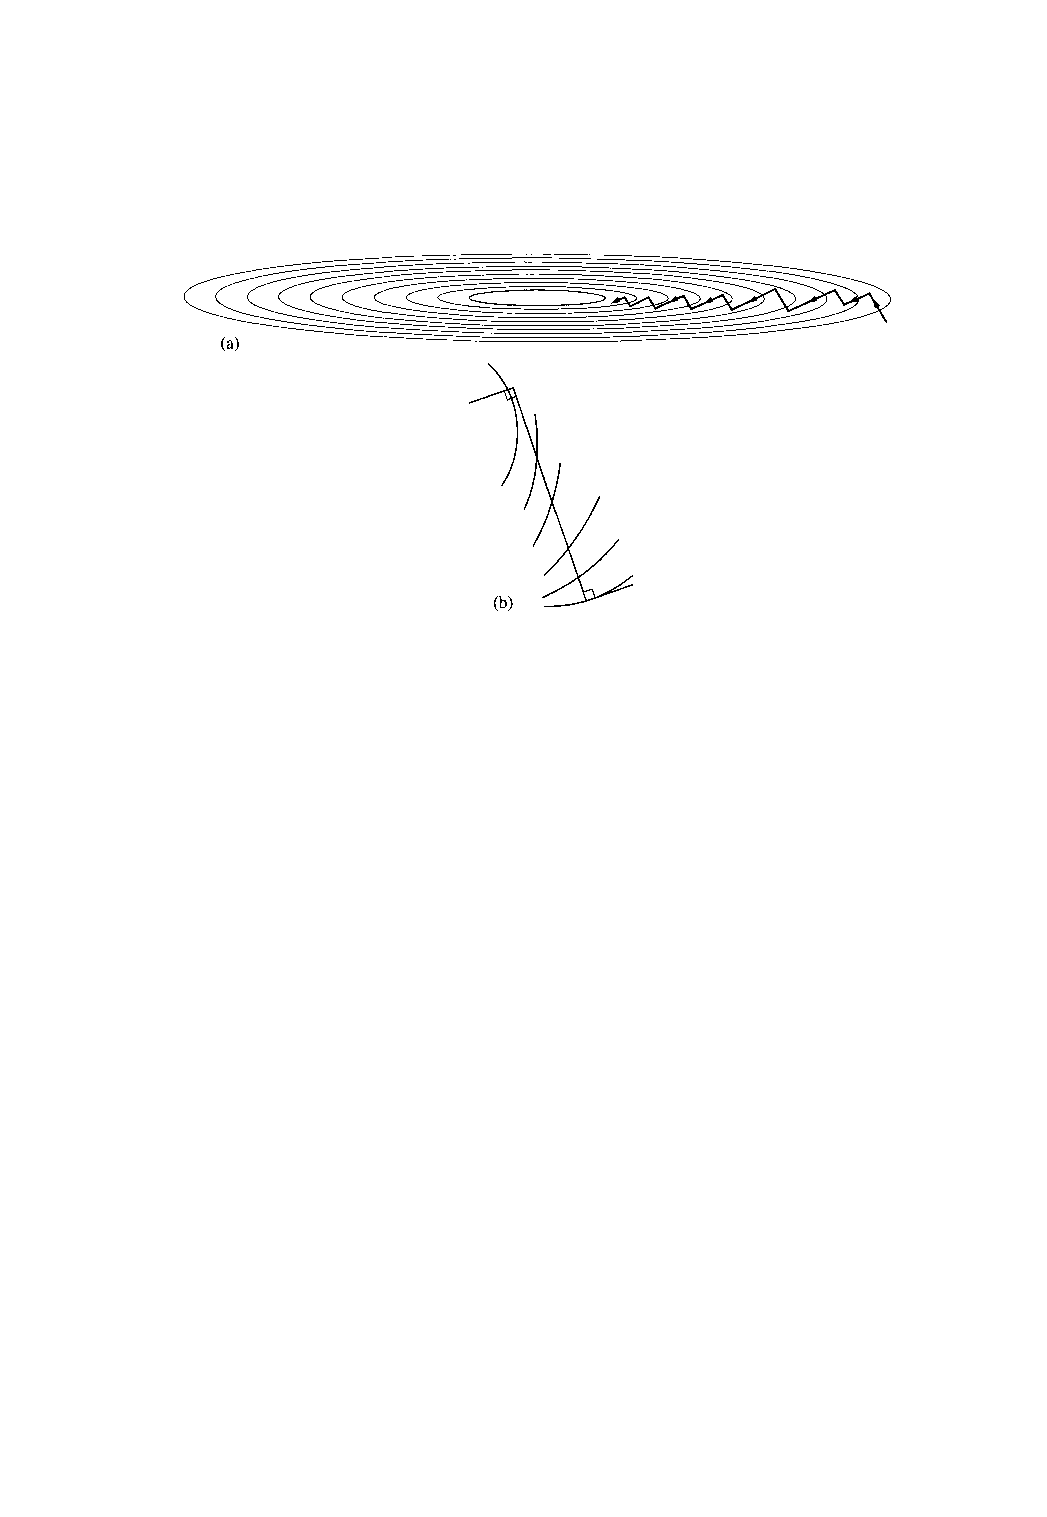
\includegraphics{image/steepest-descent.pdf}}

  \vspace*{-2em}
  \hspace*{20em}{\footnotesize(Press et al 1988)}
\end{frame}

\begin{frame}[t,fragile]{共役勾配法(conjugate-gradient)}
  \begin{itemize}
    \setlength{\itemsep}{1em}
  \item 関数がある点のまわりで
    \[
    f({\bf x}) \approx c - {\bf b}^T {\bf x} + \frac{1}{2} {\bf x}^T A {\bf x}
    \]
    と近似できるとする
  \item この時、${\bf x}$における勾配は、連立方程式$A{\bf x}={\bf b}$の「残差」の形で書ける
    \[
    -\nabla f = {\bf b} - A {\bf x}
    \]
  \item 新しい勾配方向ではなく、それまでとは「共役な方向」に進みたい
  \end{itemize}
\end{frame}

\begin{frame}[t,fragile]{「共役な方向」とは}
  \begin{itemize}
    \setlength{\itemsep}{1em}
  \item あるベクトル${\bf p}$にそった一次元の最適化が完了したとする
    \begin{itemize}
    \item その点における${\bf p}$方向の勾配は零。すなわち${\bf p}^T (\nabla f)=0$
    \item ${\bf p}$方向の勾配の値を変化させないようにしたい
  \end{itemize}
  \item 次に、${\bf q}$にそって、${\bf x}+\epsilon {\bf q}$と移動すると
    \[
      \delta(\nabla f) = A \times (\epsilon {\bf q}) \sim A {\bf q}
      \]
      これが${\bf p}$に垂直であり続けるためには
    \[
      {\bf p}^T A {\bf q} = 0
      \]
    \item この関係が成り立つ時、${\bf p}$と${\bf q}$は「互いに共役」という
  \end{itemize}
\end{frame}

\begin{frame}[t,fragile]{共役勾配法(Conjugate-gradient)}
  \begin{itemize}
    \setlength{\itemsep}{1em}
  \item 初期条件と漸化式
    \begin{align*}
      {\bf p}_0 &= {\bf r}_0 = {\bf b} - A {\bf x}_0 \\
      {\bf x}_{n+1} &= {\bf x}_n + \alpha_n {\bf p}_n \\
      {\bf r}_{n+1} &= {\bf r}_n - \alpha_n A {\bf p}_n = {\bf b} - A {\bf x}_{n+1} \\
      {\bf p}_{n+1} &= {\bf r}_{n+1} + \beta_n {\bf p}_n \\
      \alpha_n &= \frac{{\bf r}_n^T {\bf p}_n}{{\bf p}_n^T A {\bf p}_n} \ \ \
      \beta_n = \frac{{\bf r}_{n+1}^T {\bf r}_{n+1}}{{\bf r}_n^T {\bf r}_n}
    \end{align*}
  \item このように作ると、全ての$i>j \ge 1$について、自動的に
    \[
      {\bf p}_i^T A {\bf p}_j = 0 \ \ \ {\bf r}_i^T {\bf r}_j = 0
      \]
  \end{itemize}
\end{frame}

\begin{frame}[t,fragile]{共役勾配法(Conjugate-gradient)}
  \begin{itemize}
    \setlength{\itemsep}{1em}
  \item 残差は互いに直交 $\Rightarrow$ $N$回反復すると残差は零 (完全な二次形式の場合)
  \item 残差は負の勾配で表される $\Rightarrow$ $A$を知らなくても${\bf r}_i$は計算可
  \item 実際には、数値誤差により、共役性・直交性がくずれる
  \item また、完全な二次形式ではない
  \item しかし、最急降下法と比較すると圧倒的に速く収束
  \end{itemize}
\end{frame}

\begin{frame}[t,fragile]{逆反復法による固有ベクトルの計算}
  \begin{itemize}
    \setlength{\itemsep}{1em}
  \item $f(x)$の極小解は、連立一次方程式$A{\bf x} = {\bf b}$の解
    \begin{itemize}
    \item 連立方程式を解くのに共役勾配法を利用可
    \item 行列ベクトル積だけで計算できるので、$A$が疎行列の時、特に有効
    \end{itemize}
  \item 逆反復法
    \begin{itemize}
    \item 近似固有値を$\mu$とするとき、行列$(A - \mu I)^{-1}$を考えると、固有ベクトルは$A$と同じ、固有値は$(\lambda-\mu)^{-1}$。
    \item $\mu$が十分に正確であれば、$(\lambda-\mu)^{-1}$は絶対値最大の固有値。行列$(A - \mu I)^{-1}$を適当な初期ベクトルにかけ続けると$\lambda$に対応する固有ベクトルに収束(c.f. べき乗法)
    \item 実際には$(A-\mu I) {\bf x}' = {\bf x}$という連立方程式を繰り返し解く
    \end{itemize}
  \end{itemize}
\end{frame}
